\documentclass{standalone}
\usepackage{tikz}
\usepackage{mathtools}
\usepackage{pgfplots, pgfplotstable}

\pgfplotsset{compat = newest}

\definecolor{color1}{RGB}{255,158,1}
\definecolor{color2}{RGB}{255,74,1}
\definecolor{color4}{RGB}{180,0,0}

\begin{document}
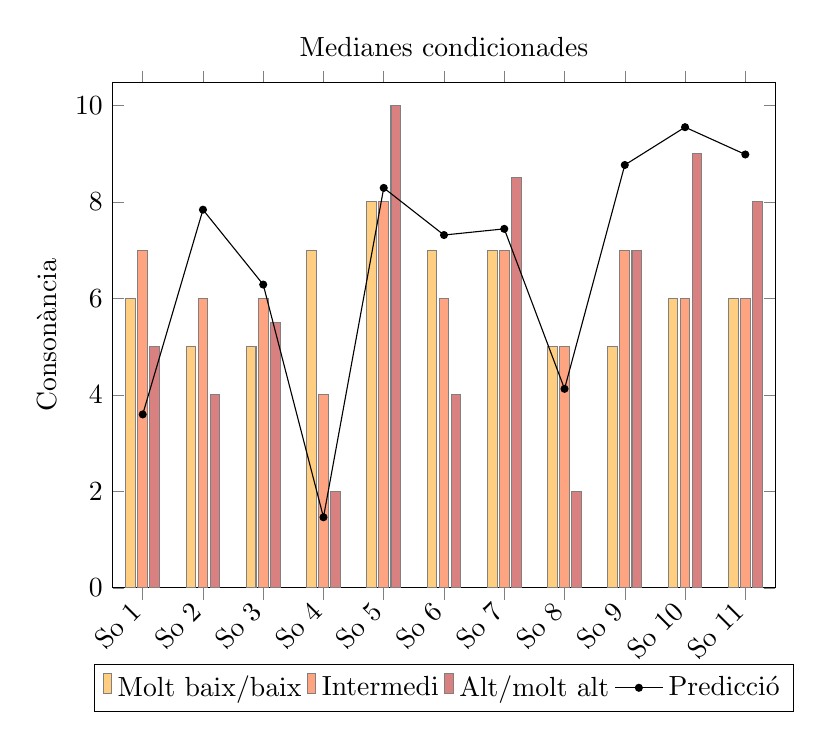
\begin{tikzpicture}
  \pgfplotsset{
    /pgfplots/ybar legend/.style={
        /pgfplots/legend image code/.code={
            \draw [##1,/tikz/.cd,bar width=3pt,yshift=-0.2em,bar shift=0pt]
            plot coordinates {(0cm,0.7em)};
          },
      },
  }
  \begin{axis}[
      title=Medianes condicionades,
      ybar=0.03cm, %sets vertical columns and shift between x-axis groups of data.
      width=10cm,
      height=8cm,
      ymin=0.475,
      ymax=10,
      xmin=So 1,
      enlargelimits=0.05, %enlarge limits of the plot
      legend style={at={(0.5,-0.15)},
          anchor=north,legend columns=-1},
      x tick label style={rotate=45,anchor=east},
      ylabel={Consonància},
      symbolic x coords={So 1,So 2,So 3,So 4,So 5,So 6,So 7,So 8,So 9,So 10,So 11},
      xtick=data,
      % nodes near coords,
      % nodes near coords align={vertical},
      bar width=3.5pt,
      % legend image code/.code={
      %     \draw [#1] (0cm,-0.1cm) rectangle (0.2cm,0.25cm); },
    ]
    \addplot[black!50,fill=color1!50] coordinates {
        (So 1,6)
        (So 2,5)
        (So 3,5)
        (So 4,7)
        (So 5,8)
        (So 6,7)
        (So 7,7)
        (So 8,5)
        (So 9,5)
        (So 10,6)
        (So 11,6)};
    \addplot[black!50,fill=color2!50] coordinates {
        (So 1,7)
        (So 2,6)
        (So 3,6)
        (So 4,4)
        (So 5,8)
        (So 6,6)
        (So 7,7)
        (So 8,5)
        (So 9,7)
        (So 10,6)
        (So 11,6)};
    \addplot[black!50,fill=color4!50] coordinates {
        (So 1,5)
        (So 2,4)
        (So 3,5.5)
        (So 4,2)
        (So 5,10)
        (So 6,4)
        (So 7,8.5)
        (So 8,2)
        (So 9,7)
        (So 10,9)
        (So 11,8)};
    \addplot[line legend,thin,mark=otimes*,sharp plot,black,mark size=1.25pt] coordinates {
        (So 1,3.595)
        (So 2,7.839)
        (So 3,6.287)
        (So 4,1.463)
        (So 5,8.291)
        (So 6,7.314)
        (So 7,7.442)
        (So 8,4.125)
        (So 9,8.766)
        (So 10,9.55)
        (So 11,8.984)}; %Some available options inside [...]: mark=square*,otimes*,triangle*,diamond*,*,square*,otimes*,star,diamond*
    \legend{Molt baix/baix,Intermedi,Alt/molt alt,Predicció}
  \end{axis}
\end{tikzpicture}
\end{document}
